\chapter{Jets data}
\label{ch:jets}
In this Chapter, base on Ref.~\cite{AbdulKhalek:2020jut}, we present a systematic analysis for the inclusion 
of jets cross-sections in a global parton distributions determination,
assessing the impact of jets and dijets production measurements on the PDFs at various perturbative orders.

% 
There is a number of unsettle theoretical issues regarding the choice of the most suitable jets observable
to be considered for precision QCD studies, such as for example the determination of PDFs,
On one hand, the simplest inclusive observable, 
the single-inclusive jets cross-section~\cite{Ellis:1990ek,Aversa:1988fv}, turns out to be non-unitary.
A possible alternative free from this issue is offered by the dijets cross-section which however, despite appearing to be 
especially well suited for PDFs determination~\cite{Giele:1994xd}, at NLO displays a significant scale dependence. 
Thanks to the recent NNLO computation for these observables, this last problem has essentially been settled,
with the scale dependence of dijets cross-section being under control at NNLO.
On the other hand, the single-jet inclusive cross section
shows a scale dependence which is not reduced when going to NNLO~\cite{Currie:2017ctp}, 
showing how the perturbative behaviour, the scale dependence~\cite{Currie:2018xkj} and even the definition~\cite{Cacciari:2019qjx} 
of this observable are non-trivial.  

%
In this study we address these issues in the context of PDFs determination, studying the impact of both single-inclusive
jets and dijets cross-sections with different scale choices in a global parton distributions fit. 
This allows us to asses which observable and scale choice leads to better PDFs compatibility with other data, better fit quality,
and more stringen constraint on the parton distributions, and provides a guideline for the inclusion of jets observables in a future
global fit (NNPDF4.0).

\section{Jets data from ATLAS and CMS}
The ATLAS and CMS collaborations have performed a number of measurements of single-inclusive and 
dijets cross sections, with center of mass energies ranging from $\sqrt{s}=2.76$ to $13$ TeV.
In this work we will consider single-inclusive and dijets data at $\sqrt{s}=7$ and $8$ TeV.
%
Whereas recent global PDFs determinations include some jets data, like for instance NNPDF3.1, which includes ATLAS and CMS 
single-inclusive data with $\sqrt{s}=2.76$ and $7$ TeV, this is the first time that the full LHC-Run I jet dataset is being 
considered. In particular dijets data have not been included in any other previous analysis.

%
The specific features of the data considered here are summarized in Table~\ref{tab:input_datasets}:
for each dataset we reported the centre of mass energy $\sqrt{s}$, 
the integrated luminosity $\mathcal{L}$, the jet radius $R$,
the measured differential distribution and the number of datapoints $n_{\text{dat}}$.
The relevant kinematic variables are defined as follows.
For single-inclusive jets we denote as $p_T$ and $y$ the transverse momentum and rapidity.
For dijets, $m_{jj}$ is the invariant dijet mass, $y^*$ and $|y_{\text{max}}|$ are the absolute rapidity difference
and the maximum absolute rapidity of the two leading jets of the event, defined as $y^*=|y_1-y_2|/2$
and $|y_{\text{max}}|= \text{max}\left(|y_1|,|y_2|\right)$ respectively.
Finally, considering the dijets triple differential distribution,
$p_{T,\rm avg} = \left(p_{T_1}+p_{T_2}\right)/2$ is the average transverse momentum of the two leading jets and 
$y_b = |y_1+y_2|/2$ is the boost of the dijets system.

%
The ATLAS 7 TeV data for single-inclusive jet, given as distributions differential in transverse momentum 
$p_T$ and rapidity $y$, cover the kinematic range $100\,\, \text{GeV} \leq p_T \leq 1.992\,\, \text{TeV}$,
$0 \leq |y| \leq 3$, while the ATLAS 8 TeV data cover the same range in rapidity but with an extended transverse momentum
kinematic coverage $70\,\, \text{GeV} \leq p_T \leq 2.5\,\, \text{TeV}$.
In our default fit we include only the central rapidity bin ($y_{jet} \leq 0.5$) of ATLAS 7 TeV, 
for ease of comparison with the NNPDF3.1 analysis of Ref.~, where the same choice was adopted due to
the difficulty in achieving a good description of the complete set of rapidity bins using
the default experimental covariance matrix\footnote{In Refs.~\cite{Ball:2017nwa,Nocera:2017zge} this choice was validated,
showing how PDFs determined from each rapidity bin in turn are indistinguishable.}.
The CMS 7 TeV data are available for $100\,\, \text{GeV} \leq p_T \leq 2.0\,\, \text{TeV}$,
$0 \leq |y| \leq 2.5$, and the CMS 8 TeV cover the extended
ranges $74\,\, \text{GeV} \leq p_T \leq 2.5\,\, \text{TeV}$ and $0 \leq |y| \leq 3.0$.

%
Moving to dijets cross-sections, in the case of ATLAS 7 TeV the measurements are double-differential in
$m_{jj}$ and $|y^*|$, with
$260\,\,\text{GeV}\leq m_{jj} \leq 4.27\,\,\text{TeV}$ and $0 \leq y^* \leq 3.0$, while for CMS 7 TeV
the distributions are differential in  $m_{jj}$ and $|y_{\text{max}}|$, with
$200\,\,\text{GeV}\leq m_{jj} \leq 5\,\,\text{TeV}$ and $0 \leq |y_{\text{max}}| \leq 2.5$.  
Finally the CMS 8 TeV data are triple-differential in $p_{T,\rm avg}$, $y_b$ and $y^*$ with
ranges $133\,\,\text{GeV} \leq p_{T,\rm avg} \leq 1.78\,\,\text{TeV}$ and $0\leq y_b,\,y^* \leq 3$.
Note that ATLAS dijets measurements are currently available at 7 and 13 TeV bit not at 8 TeV.

%
In addition to the datasets listed in Table~\ref{tab:input_datasets} ATLAS and CMS have performed
measurements at $\sqrt{s}=13$ TeV for both single-inclusive jet~\cite{Aaboud:2017wsi,Khachatryan:2016wdh}
and dijets~\cite{Aaboud:2017wsi,Sirunyan:2020uoj}. These however have smaller integrated luminosities, for this reason
we do not include these datasets in the analysis. 
%
Finally several measurements for multijets production are also available, with ATLAS providing differential distributions for
three jets cross-sections at 7 TeV~\cite{Aad:2014rma} and four jets cross-sections at 8 TeV~\cite{Aad:2015nda} 
and CMS for three jets at 7 TeV~\cite{CMS:2014mna}.
However theoretical predictions for these observables are currently available only up to NLO, and therefore they will
not be considered here.

%
For all the measurements considered here, the complete set of systematic uncertainties and correlations available from
{\tt HepData} have been used.

%-------------------------------------------------------------------------------
\begin{table}[!t]
    \centering
    \scriptsize
    \renewcommand{\arraystretch}{1.90}
    %-------------------------------------------------------------------------------
\begin{tabularx}{\textwidth}{XXcccccc}
\toprule
  Experiment 
& Measurement   
& $\sqrt{s}$ [TeV]
& $\mathcal{L}$ [fb$^{-1}$] 
& $R$
& Distribution  
& $n_{\rm dat}$ 
& Reference   \\
\midrule
  ATLAS  
& Inclusive jets  
& 7 
& 4.5
& 0.6
& $d^2\sigma/dp_Td|y|$  
& 140  
& \cite{Aad:2014vwa}  \\
  CMS  
& Inclusive jets  
& 7
& 4.5
& 0.7
& $d^2\sigma/dp_Td|y|$  
& 133 
& \cite{Chatrchyan:2012bja}  \\
  ATLAS  
& Inclusive jets  
& 8
& 20.2
& 0.6
& $d^2\sigma/dp_Td|y|$  
& 171  
& \cite{Aaboud:2017dvo}  \\
  CMS  
& Inclusive jets  
& 8 
& 19.7
& 0.7
& $d^2\sigma/dp_Td|y|$  
& 185  
& \cite{Khachatryan:2016mlc}  \\
\midrule
  ATLAS  
& Dijets  
& 7 
& 4.5
& 0.6
& $d^2\sigma/dm_{jj}d|y^{*}|$  
& 90 
& \cite{Aad:2013tea}  \\
  CMS  
& Dijets  
& 7 
& 4.5
& 0.7
& $d^2\sigma/dm_{jj}d|y_{\rm max}|$  
& 54  
& \cite{Chatrchyan:2012bja}  \\
  CMS  
& Dijets  
& 8 
& 19.7
& 0.7
& $d^3\sigma/dp_{T,\rm avg}dy_b dy^{*}$  
& 122  
& \cite{Sirunyan:2017skj}  \\
\bottomrule
\end{tabularx}
%------------------------------------------------------------------------------ 

    \vspace{0.3cm}
    \caption{\small The LHC single-inclusive jet and dijet cross-section data
       that will be used  in this study. For each dataset we indicate the experiment,
       the measurement, the center of mass energy $\sqrt{s}$, the luminosity 
       $\mathcal{L}$, the jet radius $R$, the measured distribution, the number of 
       datapoints $n_{\rm dat}$ and the reference.}
    \label{tab:input_datasets}
\end{table}
%-------------------------------------------------------------------------------
    


\section{Theoretical calculations}
In this section we present the main aspects of the theoretical calculations used to perform
our phenomenological study, discussing scale choices and QCD corrections up to NNLO.
\comment{I would exclude discussion of EW corrections, maybe I could put in an appendix}

%
As mentioned at the beginning of this chapter, even when considering NNLO predictions
the single-inclusive jet cross-sections are in general
rather sensible to the choice of central scale.
Three possible choices are given by the individual jet transverse momentum $p_T$, 
the leading jet transverse momentum $p_{T,1}$ and the scalar sum of the transverse momenta of all the partons
in the event 
\begin{align}
    \hat{H}_T = \sum_{i\in\text{partons}} p_{T,i}\,.
\end{align}
Predictions obtained from different scales choices may differ, even at NNLO, by amounts which are comparable to their
scale dependence.
In Ref.~\cite{Currie:2018xkj} the scales $\mu = \hat{H}_T $ and $\mu = 2p_T$ were singled out as optimal ones,
according to a number of criteria, such as perturbative convergence and scale uncertainty as error estimate.
Here we will consider results for $\mu = \hat{H}_T$, which will be compared to those found using $\mu=p_T$,
which was the baseline choice adopted in previous NNPDF dterminations.

%
Turning to dijets observables, also here different scale choices are possible. As mentioned before, at NLO theoretical predictions
computed with different choices differ significantly, however the problem is alleviated at NNLO, with $\mu = m_{jj}$
emerging as preferred choice~\cite{Currie:2017eqf,Currie:2018oxh}, which therefore will be adopted here. 

%
As detailed in Chapter~\ref{ch:nnpdf_methodology}, the partonic matrix elements entering a PDFs fit
have to be precomputed in such a way that the numerical convolution with generic input PDFs can be approximated by mean
of interpolation techniques. 
To this purpose we use {\tt NLOJET++}~\cite{Nagy:2001fj} interfaced to {\tt F{\small AST}NLO}~\cite{Wobisch:2011ij}.
The computation is performed using the scale choices described above and is validated against the {\tt NNLOJET} computation.
This fast interpolation grids are then combined with PDF evolution kernel using {\tt APFEL{\small GRID}}~\cite{Bertone:2016lga}
to obtain FK tables, as described in Eq.~\ref{eq:DY_obs}.
However fast interpolation grids to be used as input for {\tt APFEL{\small GRID}} are available only at NLO.
We therefore implement NNLO QCD corrections by supplementing the NLO grids with QCD $K$-factors as detailed in the following.
We computed exact NNLO QCD predictions using {\tt NNLOJET}~\cite{Gehrmann-DeRidder:2019ibf} and we define the 
corresponding $K$-factors as
\begin{align}
    \label{eq:QCD_kfactors}
    K^{\text{QCD}}_{\text{NNLO}} = \frac{\sum_{ij}\hat{\sigma}_{ij}^{\text{NNLO}}\otimes \mathcal{L}_{ij}^{\text{NNLO}}}
    {\sum_{ij}\hat{\sigma}_{ij}^{\text{NLO}}\otimes \mathcal{L}_{ij}^{\text{NNLO}}}\,,
\end{align}
where the sum runs over partonic subchannels, $\hat{\sigma}_{ij}$ are partonic matrix elements and $\mathcal{L}$
the corresponding parton luminosity, computed in both the numerator and denominator using NNPDF3.1 NNLO as a fixed input 
PDF set.
NNLO grids for the relevant cross-sections are then obtained from the corresponding NLO grids through the multiplicative
prescription
\begin{align}
    \label{eq:NNLO_kfactors}
    \frac{d^2\sigma}{dp_T dy}\Bigg|_{NNLO} = \frac{d^2\sigma}{dp_T dy}
    \Bigg|_{\rm NLO_{QCD}} \times K_{\rm NNLO}^{\rm QCD}(p_T,y,\sqrt{s})\, .
\end{align}
The first term on the right-hand side is the output of the NLO computation, given in terms of fast interpolation grids,
while the second term is the bin-by-bin QCD $K$-factors computing according to Eq.~\ref{eq:QCD_kfactors}. 
The result is validated against the full NNLO result from {\tt NNLOJET}. In general QCD $K$-factors might be affected by 
point-to-point fluctuations due to underlying numerical uncertainties affecting the NNLO computation,
therefore they are provided with a Monte Carlo uncertainty, estimated as described in Ref.~\cite{Ridder:2016rzm}.
This uncertainty is added in quadrature to the experimental one when performing the PDFs fit, fully uncorrelated datapoint 
by datapoint.
For illustration purpose, NNLO QCD $K$-factors for the central rapidity bins $0\leq |y| \leq 0.5$
of thevATLAS 7 TeV single-inclusive jet and of the CMS 8 TeV dijet distributions are displayed 
in Fig.~\ref{fig:kfactqcd_werrors} as functions of $p_T$, together with the corresponding Monte Carlo uncertainties.
In both cases the NNLO QCD $K$-factors increase monotonically with $p_T$ from about $5\%$ to about $20\%$ for single-inclusive
jets, and from about $3\%$ to $15\%$ for dijets. 
\begin{figure}[!t]
    \centering
    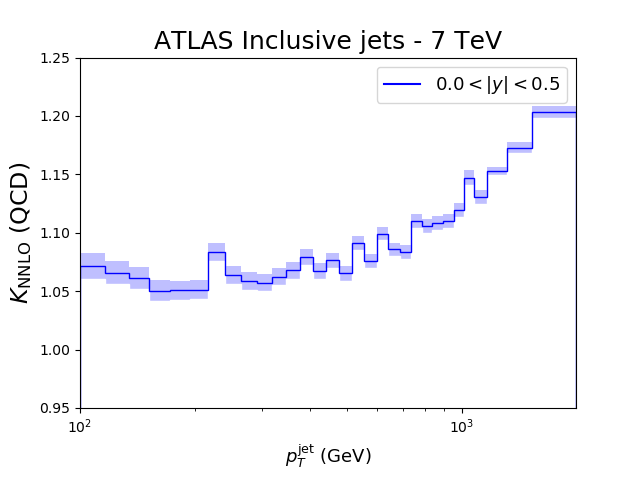
\includegraphics[scale=0.44]{kfactqcd_incljets_atlas7_HTp_R06-rap1-werrors-hist.png}
    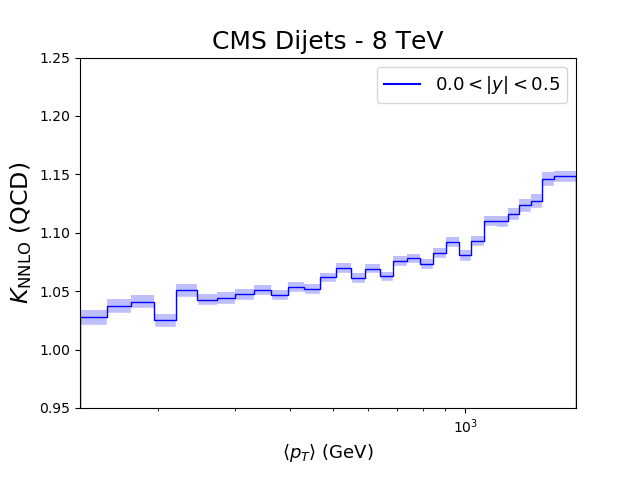
\includegraphics[scale=0.44]{kfactqcd_dijets_cms8_mjj_R07-rap1-werrors-hist.png}
    \caption{The NNLO QCD $K$-factors for the central rapidity bins of the ATLAS 
       7~TeV single-inclusive jets (left) and CMS 8~TeV dijets (right), with
       the Monte Carlo numerical uncertainties shown as filled bands around the 
       central result.}
\label{fig:kfactqcd_werrors} 
\end{figure}



\section{Results}

\begin{table}[!t]
    \renewcommand*{\arraystretch}{1.60}
    \scriptsize
    \centering
    %-------------------------------------------------------------------------------
\begin{tabularx}{\textwidth}{Xlll}
    \toprule
    & NNLO$_{\rm QCD}$+EW
    & NNLO$_{\rm QCD}$
    & NLO$_{\rm QCD}$\\
    \midrule
    baseline (see text)                           &  ---      &  bn     & b    \\
    \midrule
    ATLAS \& CMS jets   7-8~TeV                   & janw      & ---    & ---   \\
    ATLAS \& CMS jets   7~TeV                     & j7nw      & j7n    & j7    \\
    ATLAS \& CMS jets   7~TeV ($\mu=p_T^{\rm jet}$) &  ---      & j7n-pt & j7-pt \\
    ATLAS \& CMS jets   8~TeV                     & j8nw      & j8n    & j8    \\
    \midrule
    ATLAS \& CMS dijets 7-8~TeV                   & danw      & ---    & ---   \\
    ATLAS \& CMS dijets 7~TeV                     & d7nw      & d7n    & d7    \\
    CMS          dijets 8~TeV                     & d8nw      & d8n    & d8    \\
    \bottomrule
    \end{tabularx}
    %-------------------------------------------------------------------------------
    \vspace{0.3cm}
    \caption{The PDF determinations discussed in this study and their
      IDs. Each row corresponds to a different choice of input jet dataset or fit
      settings (listed in the first column), and each column corresponds
      to a different theory accuracy (listed in the first row).
      The ID encodes the process used (j for single-inclusive
      jets and d for dijets); the data used (a for all, 7 or 8 for the
      7~TeV or 8~TeV datasets); the perturbative accuracy (n for QCD NNLO); and the choice of scale (pt when
      $\mu=p_T^{\rm jet}$).
      In this and subsequent tables and plots
      ``jets'' is short for single-inclusive jets.}
    \label{tab:listfits}
\end{table}

\begin{table}[t]
    \renewcommand*{\arraystretch}{1.60}
    \scriptsize
    \centering
    %-------------------------------------------------------------------------------
\begin{tabularx}{\textwidth}{Xrcccc}
    \toprule
     Dataset                    & $n_{\rm dat}$ &    bn   &  janw  &      j7nw  &      j8nw  \\
    \midrule
     DIS NC                     &       2103  &    1.17  &  1.18  &    1.17  &    1.18  \\
     DIS CC                     &        989  &    1.10  &  1.11  &    1.10  &    1.11  \\
     Drell-Yan                  &        577  &    1.33  &  1.30  &    1.31  &    1.31  \\
     $Z$ $p_T$                  &        120  &    1.01  &  1.02  &    1.02  &    1.03  \\
     Top pair                   &         24  &    1.05  &  1.25  &    1.02  &    1.24  \\
     Jets (all)                 &        520  &  [2.60] &  1.88  &  [2.53] &  [1.89] \\
     \ \ Jets (fitted)          &             &    ---   &  1.88  &    1.12    &  2.20  \\
     \ \ ATLAS 7 TeV            &         31  &  [1.87] &  1.59  &   1.15   & [1.62] \\
     \ \ ATLAS 8 TeV            &        171  &  [5.01] &  3.22  &  [4.58]   &  3.25  \\
     \ \ CMS   7 TeV            &        133  &  [1.06] &  1.09  &    1.11   & [1.14] \\
     \ \ CMS   8 TeV            &        185  &  [1.59] &  1.25  &  [1.80]   &  1.23  \\
     Dijets (all)               &        266  &  [3.07] & [2.10] &  [2.56]  & [2.22] \\
     \ \ Dijets (fitted)        &             &    ---   &  ---   &    ---      &  ---   \\
     \ \ ATLAS 7 TeV            &         90  &  [2.47] & [1.95] &  [1.97]  & [2.01] \\
     \ \ CMS   7 TeV            &         54  &  [2.40] & [2.08] &  [2.12]  & [2.15] \\
     \ \ CMS   8 TeV            &        122  &  [3.81] & [2.21] &  [3.20]  & [2.39] \\
    \midrule
     Total                      &             &   1.18   &  1.28  &   1.17    &  1.27  \\
    \bottomrule
    \end{tabularx}
    %-------------------------------------------------------------------------------
    \vspace{0.3cm}
    \caption{The $\chi^2$ per datapoint for all fits of
      Table~\ref{tab:listfits} including single-inclusive jet data, with default settings.
      Results are shown
      for all datasets, aggregated by process type. For jets data, results are
      shown both for the sets included in each fit, and also for those not
      included, enclosed in square brackets. Combined results are also shown
      for all single-inclusive jet and for all dijet data, both for
      the full set, and for those included in each fit.
      The number of datapoints in each
      dataset is also shown.}
    \label{tab:chi2s}
\end{table}

\begin{table}[t]
    \renewcommand*{\arraystretch}{1.60}
    \scriptsize
    \centering
    %-------------------------------------------------------------------------------
\begin{tabularx}{\textwidth}{Xrcccc}
    \toprule
     Dataset                    & $n_{\rm dat}$ &   bn   &  danw  &  d7nw  &  d8nw  \\
    \midrule
     DIS NC                     &       2103  &  1.17  &  1.18  &  1.17  &  1.18  \\
     DIS CC                     &        989  &  1.10  &  1.12  &  1.09  &  1.12  \\
     Drell-Yan                  &        577  &  1.33  &  1.29  &  1.32  &  1.28  \\
     $Z$ $p_T$                  &        120  &  1.01  &  1.07  &  1.03  &  1.08  \\
     Top pair                   &         24  &  1.05  &  1.14  &  1.04  &  1.26  \\
     Jets (all)                 &        520  & [2.60] & [2.06] & [2.70] & [2.14] \\
     \ \ Jets (fitted)          &             &  ---   &  ---   &  ---   &  ---   \\
     \ \ ATLAS 7 TeV            &         31  & [1.87] & [1.63] & [1.74] & [1.61] \\
     \ \ ATLAS 8 TeV            &        171  & [5.01] & [3.36] & [4.65] & [3.55] \\
     \ \ CMS   7 TeV            &        133  & [1.06] & [1.06] & [1.14] & [1.07] \\
     \ \ CMS   8 TeV            &        185  & [1.59] & [1.64] & [2.17] & [1.68] \\
     Dijets (all)               &        266  & [3.07] &  1.65  & [2.16] & [1.71] \\
     \ \ Dijets (fitted)        &             &  ---   &  1.65  &  1.72  &  1.68  \\
     \ \ ATLAS 7 TeV            &         90  & [2.47] &  1.76  &  1.78  & [1.78] \\
     \ \ CMS   7 TeV            &         54  & [2.40] &  1.60  &  1.63  & [1.66] \\
     \ \ CMS   8 TeV            &        122  & [3.81] &  1.58  & [2.67] &  1.68  \\
    \midrule
     Total                      &             &  1.18  &  1.22  &  1.19  &  1.20  \\
    \bottomrule
    \end{tabularx}
    %-------------------------------------------------------------------------------
    \vspace{0.3cm}
    \caption{Same as Table~\ref{tab:chi2s}, but now for dijets. The
      baseline is repeated for ease of reference.}
    \label{tab:chi2sD}
\end{table}

\begin{table}[!t]
    \renewcommand*{\arraystretch}{1.60}
    \scriptsize
    \centering
    \begin{tabularx}{\textwidth}{Xrccc}
    \toprule
     Dataset                    & $n_{\rm dat}$ & janw &    janw-8dec   &  janw-8pcor     \\
    \midrule
     \ \ ATLAS 7 TeV            &         31  & 1.59 &  1.59 &  1.61     \\
     \ \ ATLAS 8 TeV            &        171  & 3.22 &  0.83 &  0.98     \\
     \ \ CMS   7 TeV            &        133  & 1.09 &  1.12 &  1.12     \\
     \ \ CMS   8 TeV            &        185  & 1.25 &  1.42 &  1.42     \\
     \ \ ATLAS 7 TeV            &         90  & [1.95] & [1.98] & [1.98]    \\
     \ \ CMS   7 TeV            &         54  & [2.08] & [2.19] & [2.17]    \\
     \ \ CMS   8 TeV            &        122  & [2.21] & [2.96] & [3.04]    \\
    \bottomrule
\end{tabularx}
    %-------------------------------------------------------------------------------
    \vspace{0.3cm}
    \caption{Same as Table~\ref{tab:chi2s} for
      fits performed with alternative choices of central
      scale. Now only $\chi^2$ values
      for jet data are shown. Results for the fits with default settings
      \#j7 and \#j7n  already shown  in Table~\ref{tab:chi2s} are included
      for ease of reference.}
    \label{tab:chi2_suppl}
\end{table}